\documentclass[12,a4paper]{article}

\usepackage{graphicx}
\usepackage{float}
\usepackage{caption}
\usepackage{subcaption}
\usepackage{amsmath}
\usepackage{listings}
\usepackage{color}
\usepackage{array}
\newcolumntype{P}[1]{>{\centering\arraybackslash}p{#1}}

\definecolor{dkgreen}{rgb}{0,0.6,0}
\definecolor{gray}{rgb}{0.5,0.5,0.5}
\definecolor{mauve}{rgb}{0.58,0,0.82}

\def\code#1{\texttt{#1}}

\lstset{
  language=C++,
  aboveskip=3mm,
  belowskip=3mm,
  showstringspaces=false,
  columns=flexible,
  basicstyle={\small\ttfamily},
  numbers=none,
  numberstyle=\tiny\color{gray},
  keywordstyle=\color{blue},
  commentstyle=\color{dkgreen},
  stringstyle=\color{mauve},
  breaklines=true,
  breakatwhitespace=true,
  tabsize=3
}

\title{High Performance Computing}
\date{\today}
\author{Amarnath Karthi  201501005 \\ Chahak Mehta  201501422}

\setlength{\parindent}{0em}

\makeatletter
\begin{document}
    \begin{titlepage}
	\centering
	{\scshape\LARGE CS-301 \par}
	\vspace{0.1cm}
	{\huge \@title \par}
	\vspace{0.5cm}
	{\Large Assignment 6\par}
	\vspace{10cm}
	\Large Amarnath Karthi          201501005\\
	\Large Chahak Mehta             201501422\\
	\vspace{5cm}
	{\large \@date\par}
    \end{titlepage}
    
    
    \section{Hardware and Compiler specifications}
    \renewcommand{\arraystretch}{1.5}
    \begin{table}[H]
        \centering
        \begin{tabular}{ |P{0.4\textwidth}|P{0.6\textwidth}|}
            \hline
            \textbf{Architecture} & x86\_64\\
            \hline
            \textbf{CPU op-mode(s)} & 32-bit, 64-bit\\
            \hline
            \textbf{Byte Order} & Little Endian\\
            \hline
            \textbf{CPU(s)} & 12\\
            \hline
            \textbf{On-line CPU(s) list} & 0-11\\
            \hline
            \textbf{Thread(s) per core} & 1\\
            \hline
            \textbf{Core(s) per socket} & 6\\
            \hline
            \textbf{Socket(s)} & 2\\
            \hline
            \textbf{NUMA node(s)} & 2\\
            \hline
            \textbf{Vendor ID} & GenuineIntel\\
            \hline
            \textbf{CPU family} & 6\\
            \hline
            \textbf{Model} & 63\\
            \hline
            \textbf{Model name} & Intel(R) Xeon(R) CPU E5-2620 v3 @ 2.40GHz\\
            \hline
            \textbf{Stepping} & 2\\
            \hline
            \textbf{CPU MHz} & 1211.531\\
            \hline
            \textbf{BogoMIPS} & 4804.10\\
            \hline
            \textbf{Virtualization} & VT-x\\
            \hline
            \textbf{L1d cache} & 32K\\
            \hline
            \textbf{L1i cache} & 32K\\
            \hline
            \textbf{L2 cache} & 256K\\
            \hline
            \textbf{L3 cache} & 15360K\\
            \hline
            \textbf{NUMA node0 CPU(s)} & 0-5\\
            \hline
            \textbf{NUMA node1 CPU(s)} & 6-11\\
            \hline\hline
            \textbf{Language} & C\\
            \hline
            \textbf{Compiler} & mpicc\\
            \hline
        \end{tabular}
    \end{table}
    \newpage
\section{Trapezoidal Integration}
    \textbf{
        Write and analyze serial code and parallel code for the following using OpenMP.
        \begin{enumerate}
            \item Integration of a function using trapezoidal rule. Verify your code by using it to calculate the value of $\pi$.
            \item Calculation of $\pi$ using series.
            \item Summation of two vectors
        \end{enumerate}
    }
    
    \section{Solution}
    \subsection{Integration using trapezoidal rule}
    \subsubsection{Theory}
    We use the following formula to compute the value of $\pi$ :
    \begin{equation}
        \int_{0}^{1} \frac{4}{1+x^2} dx
    \end{equation}
    
    \subsubsection{Approach}
    For the serial code, we use simple numerical integration over 0 to 1 using $n$ segments for trapezoidal integration. For parallelizing we just have to divide these $n$ segments between $p$ processors and run the serial algorithm on each processor to get a local integration. After this, each processor sends the local integration answer to the master processor which adds each answer to get the global answer.
    
    This is achieved using MPI.
    
    \subsection{Sending and Receiving schemes}
    We can use 2 send receive models in MPI -
    \begin{enumerate}
        \item \textbf{MPI\_Send() , MPI\_Recv()}: Using this model, the master sends the data $n$ to each slave processor iteratively and then gets the data from each in the same manner. This is not efficient if $p$ i.e. the number of processors is large.
        \item \textbf{MPI\_Bcast(), MPI\_Reduce()}: Using this model, the master sends the data to some processors. As soon as they get the data they forward this to other processors also. This way each processor is helping in sending data, thereby reducing the communication time and increasing the bandwidth utilization. This is good if we have large number of processors.
    \end{enumerate}
    \subsubsection{Results and Observations}
    
    \begin{figure}[H]
        \centering
        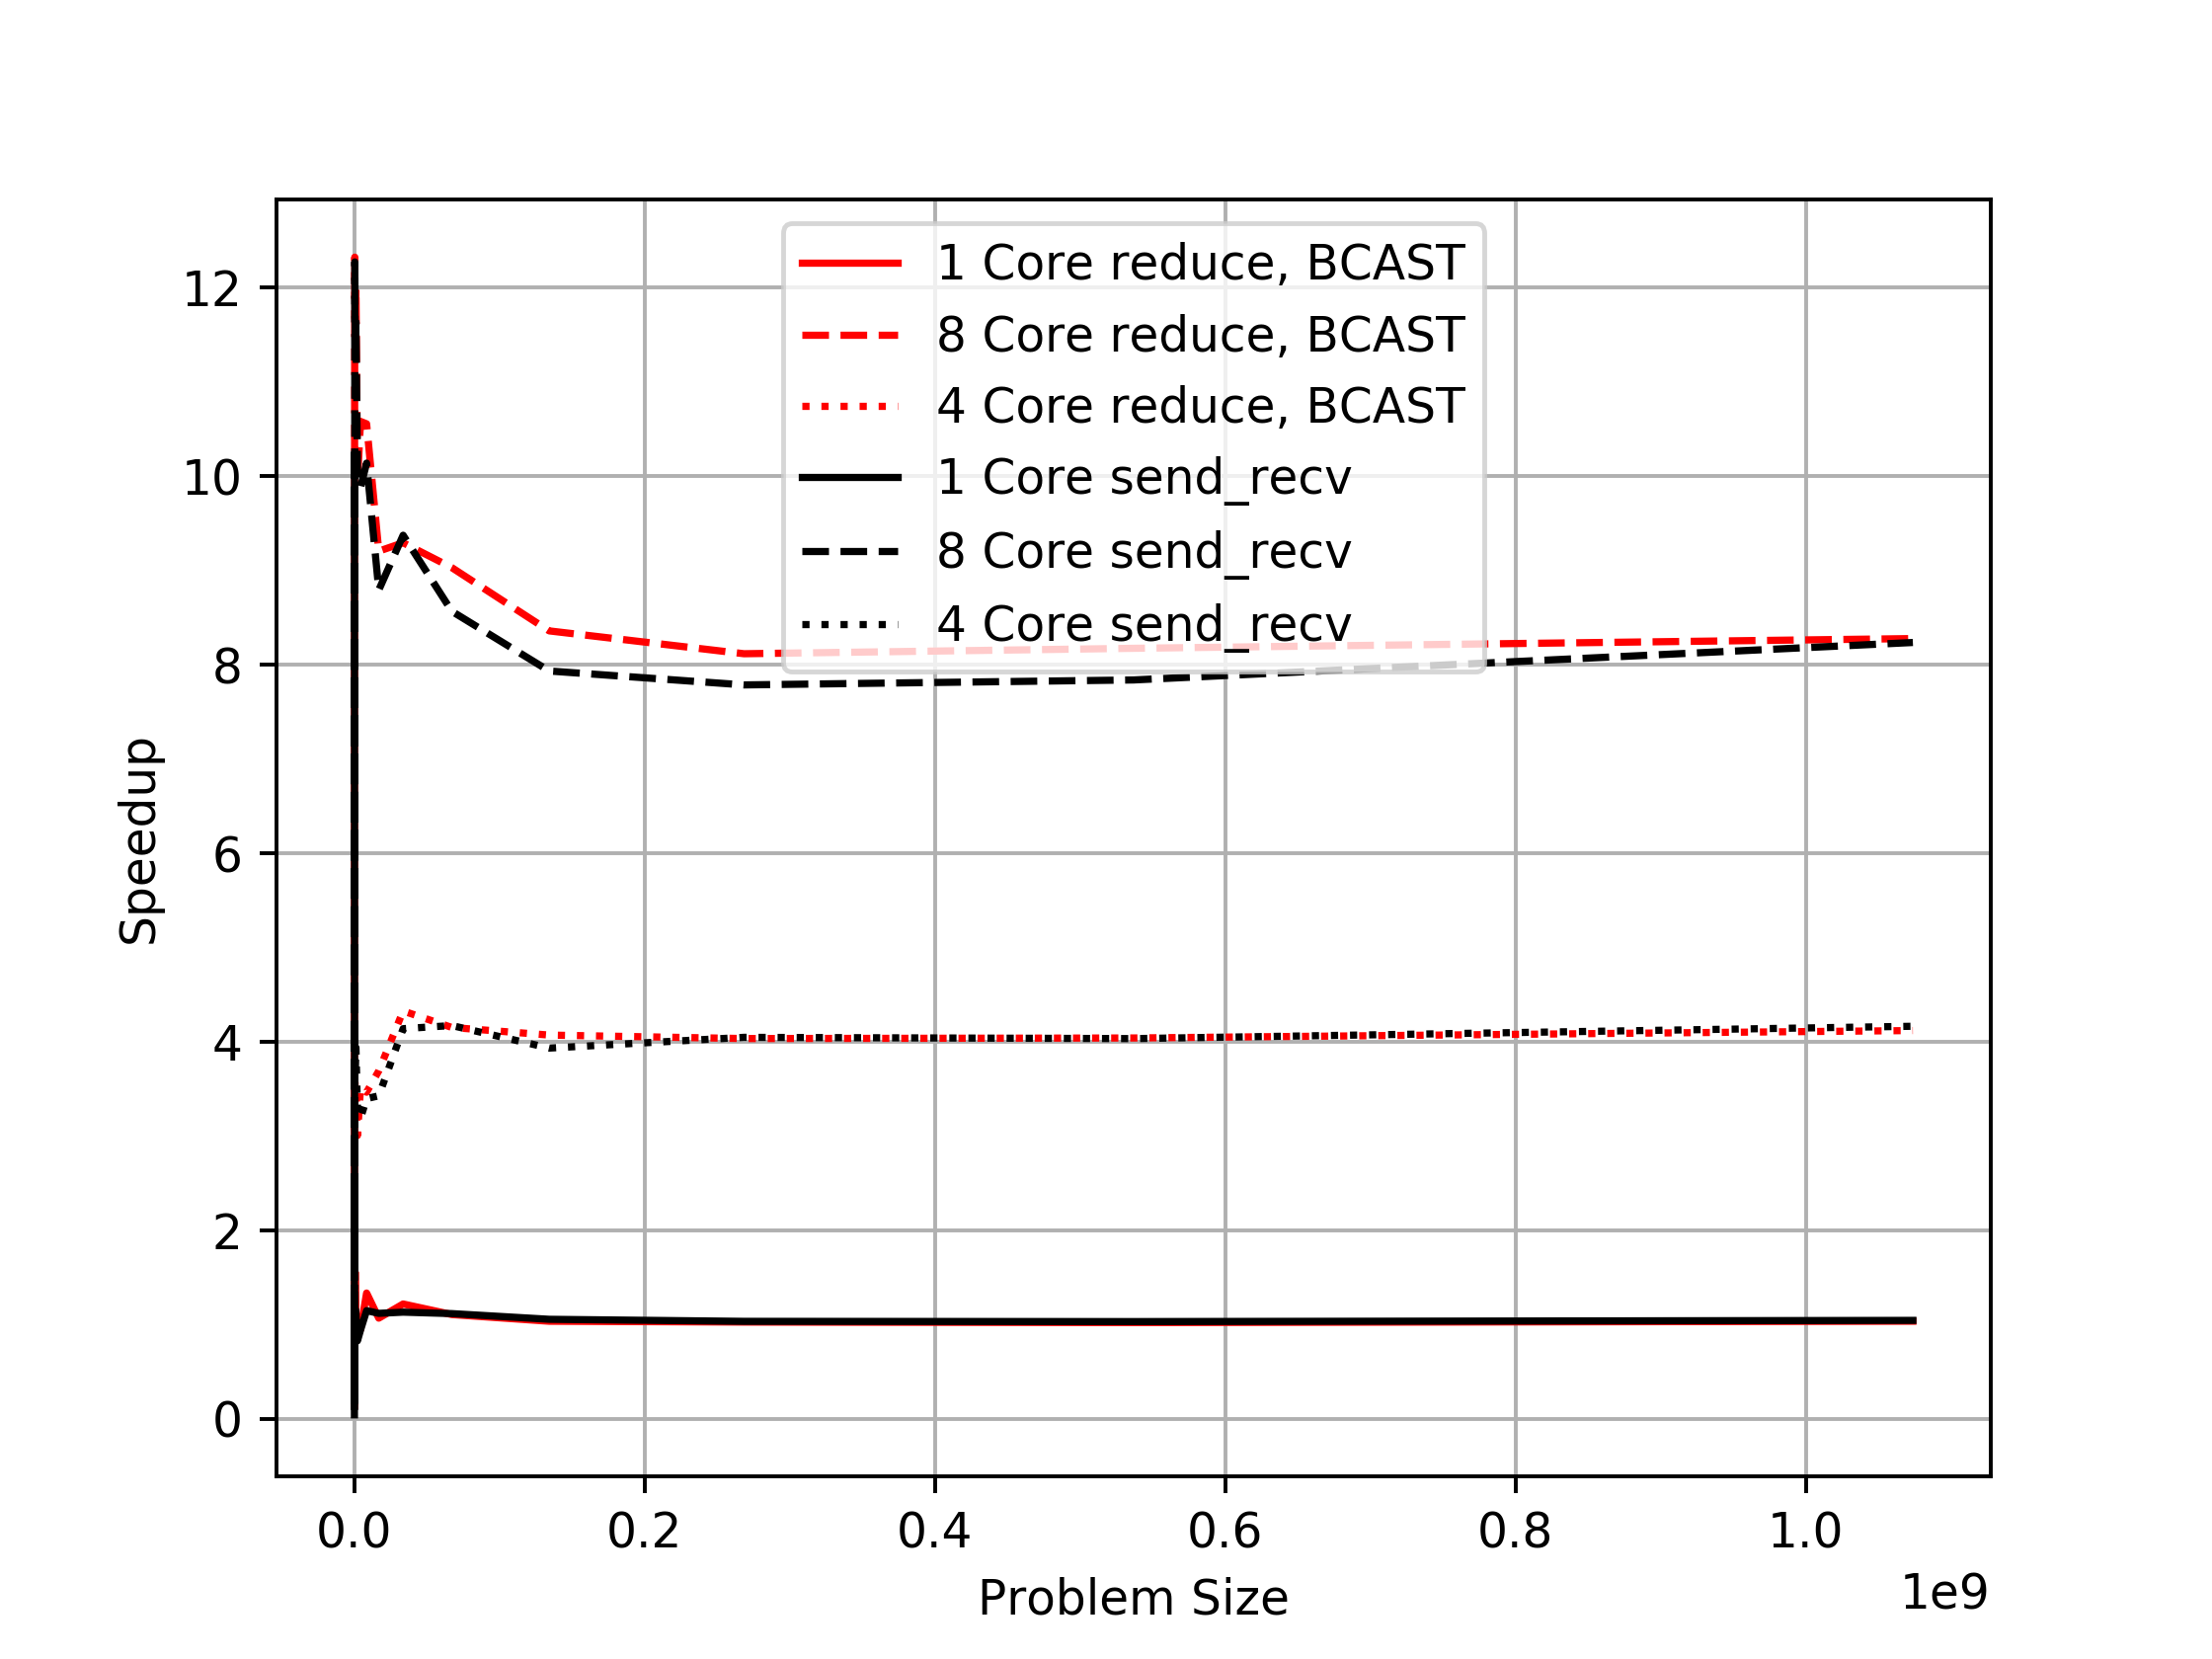
\includegraphics[width=0.8\textwidth]{plots/speedup_size.png}
        \caption{speedup vs problem size}
        \label{fig:q1p1}
    \end{figure}
    
    The above plot shows speedup as a function of number of the problem size. Notice that as we increase the number of processors, the \textbf{MPI\_Bcast()} model performs better due to the reasons mentioned in the previous section.
    
    Also there is a slight superlinear speedup so the efficiency becomes slightly greater than 1.
    
    \begin{figure}[H]
        \centering
        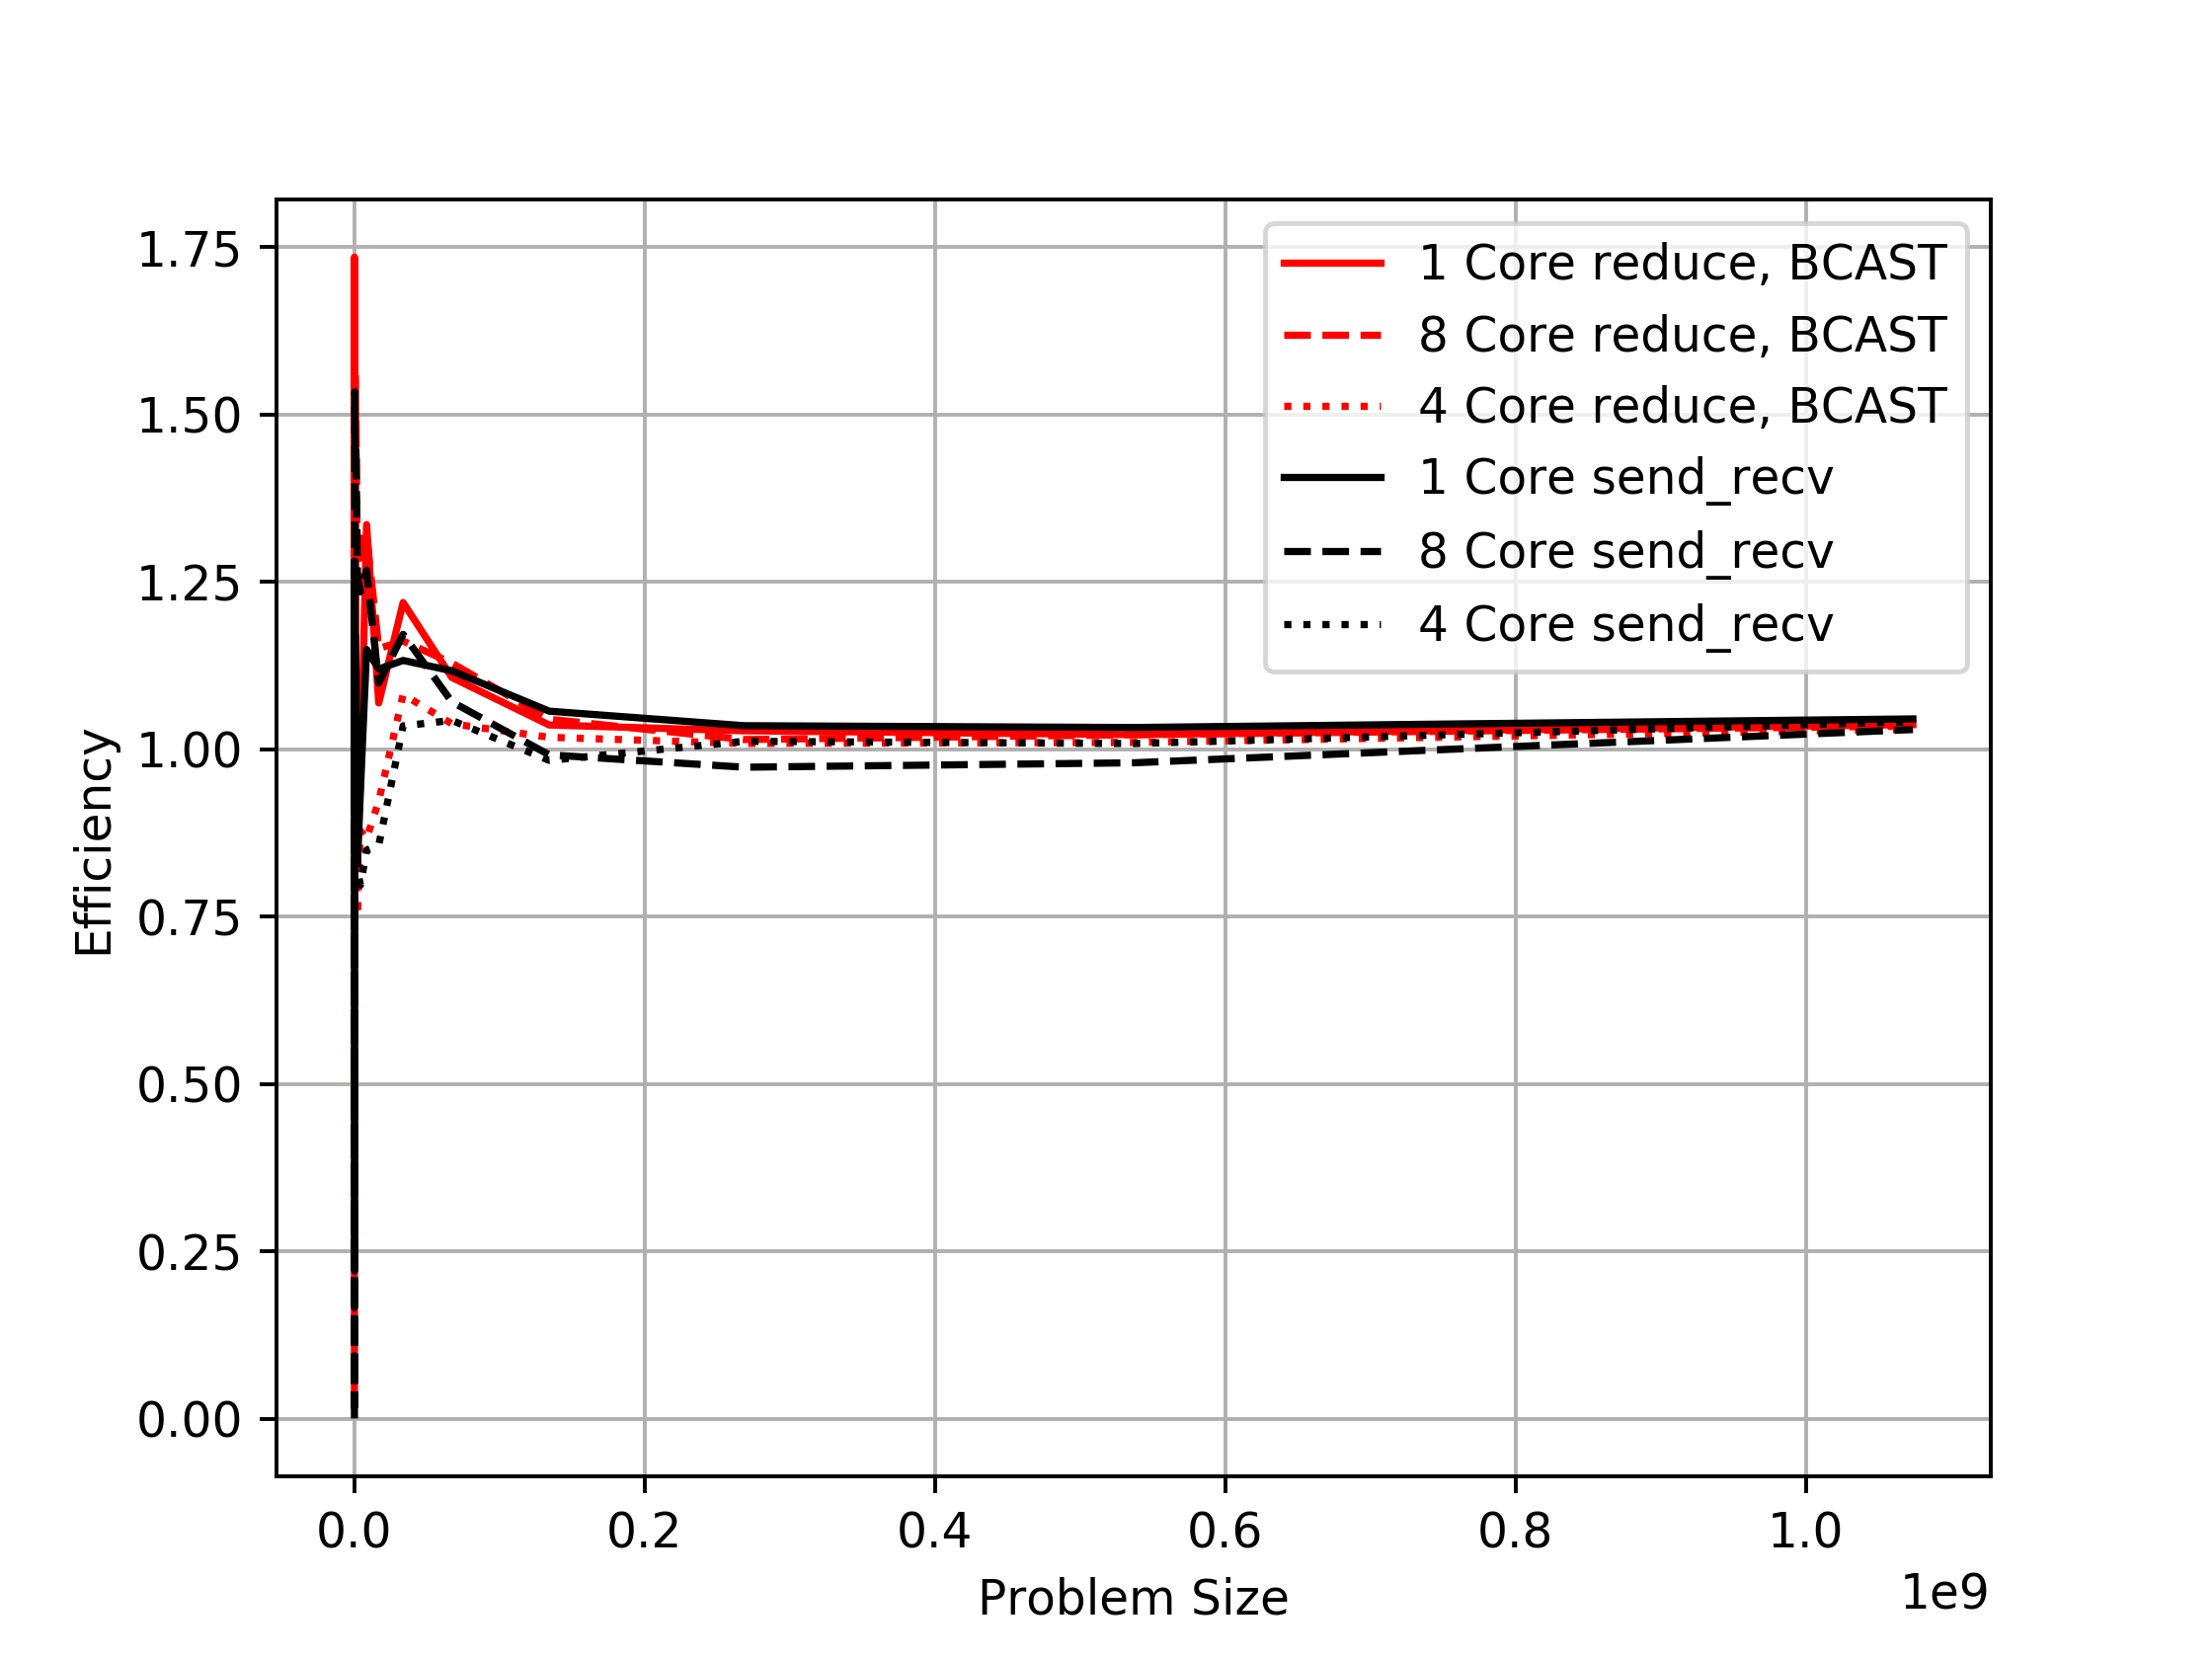
\includegraphics[width=0.8\textwidth]{plots/efficiency_size.png}
        \caption{speedup vs problem size}
        \label{fig:q2}
    \end{figure}
    \section{Matrix Multiplication}
    Perform matrix multiplication using MPI
    \subsection{Approach}
    For the following operation :
    \begin{equation}\nonumber
        AB=C
    \end{equation}
    The serial approach to evaluate C is naive matrix multiplication which runs in $O(n^3)$ time complexity. To parallelize the code, we broadcast $A$ to all processors and then decompose $B$ and distrbute it amongst $p$ processors.
    \subsection{Results and observations}
    \begin{figure}[H]
        \centering
        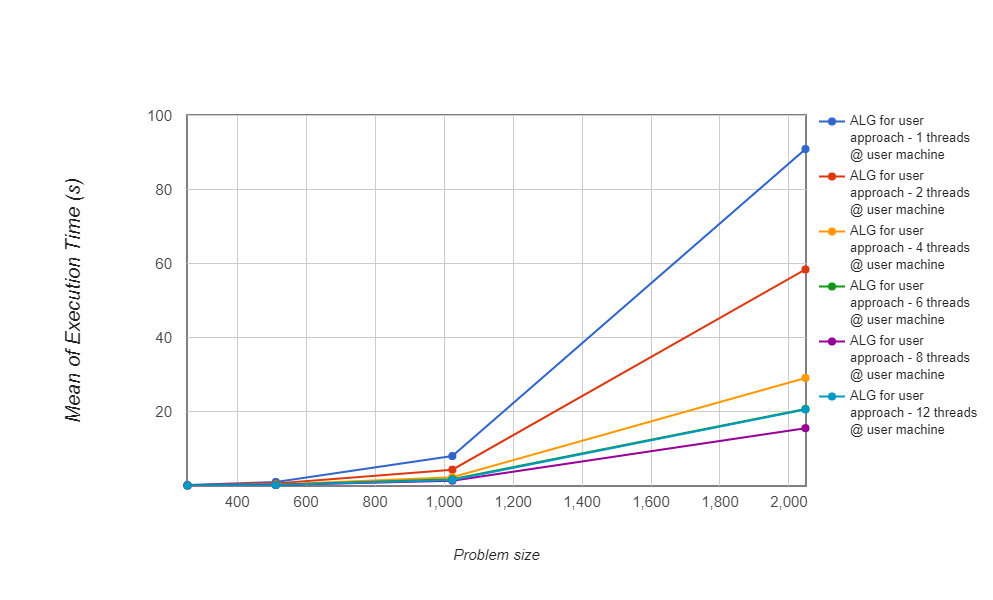
\includegraphics[width=\textwidth]{plots/mean_executionTime.png}
        \caption{Problem size vs time taken}
        \label{fig:my_label}
    \end{figure}
    The time curve is shown above for 1, 2, 4, 8 and 12 threads. Notice that 8 thread model is faster than the 12 thread model. This isbecause the inter processor communication cost is higher in 12 threads and is not compensated by the computational ease provided by the same. This can also be seen from the speedup curves shown below.
    \begin{figure}[H]
        \centering
        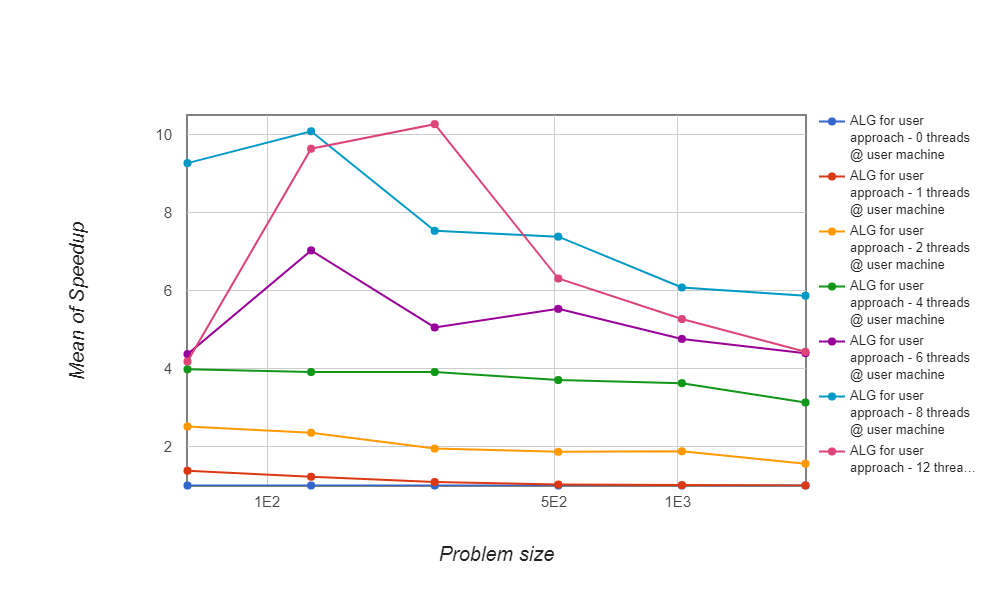
\includegraphics[width=\textwidth]{plots/mean_speedup.png}
        \caption{Problem size vs speedup}
        \label{fig:my_label}
    \end{figure}
\end{document}